\chapter{Process-Component}
	
	

Este fragmento del proyecto se dedica exclusivamente al apartado gráfico.Es una herramienta que se dedica a proveer métodos para interactuar con él, y además, es capaz mediante \emph{listeners} de avisar a los clientes que lo requieran sobre los eventos ocurridos sobre la interfaz gráfica.


Su implementación se centra en dos pilares. Por una parte se ha realizado un proyecto Vaadin encargado de mantener el estado de la aplicación gráfica, y por otro lado un conjunto de ficheros Javascript implementados sobre GO.JS que se encargan de modificar el entorno gráfico mediante sentencias .
\begin{itemize}
	\item Proyecto Vaadin
	\subitem Este proyecto es el encargado de crear los metodos necesarios para interactuar desde el exterior con el esquema creado previamente. Además debe de permitir insertar \emph{listeners} para los eventos proporcionados desde GO.JS, de forma que se pueda establecer dos direcciones de comunicación. Una desde el exterior con el proyecto Vaadin y este con el conector y directamente con el entorno gráfico de GO.JS, y otro desde interacción con los eventos (por parte del usuario) desde el fichero Javascript de configuración, con el conector y este con el estado, es decir, con el proyecto Vaadin.
	
	\item Ficheros Javascript
	\subitem Existe un primer fichero que permite configurar el esquema gráfico que se va a llevar a cabo (Procesos, Subprocesos, InputVariables, OutputVariables ...), así como todo el resto de propiedades gráficas, además de ser capaz de lanzar eventos preconfigurados.
	
	
	El segundo fichero esencial para el funcionamiento de esta estructura, es el fichero conector. Este es el encargado de declarar y configurar todos los eventos que se pueden lanzar, además de ser el encargado de realizar todos los metodos CRUD \footnote{CRUD es el acrónimo de crear, leer, actualizar y borrar, en esete contexto significa el conjunto de métodos para poder realizar dichas acciones sobre los distintos elementos existentes.}necesarios para que puedan interactuar con las propiedades configuradas en el primer fichero citado previamente.
\end{itemize}


\subsection{Ejemplo Vaadin + Javascript}

Como se explicó anteriormente, \emph{Vaadin} se encarga de abstraer al usuario del mundo Javascript, sin embargo, hay funcionalidades que \emph{Vaadin} no es capaz de alcanzar, en estos casos se utilizan componentes Javascript para enriquecer la aplicación.

El primer paso para comprender el funcionamiento de \emph{Vaadin} junto a componentes Javascript es entender su arquitectura básica. Como podemos observar en la Figura~\ref{fig:schema}, consta de tres módulos bien diferenciados. El primer módulo se corresponde con el proyecto implementado en Java. El segundo con el conector en javascript que servirá de comunicador o intermediario entre la librería Javascript y el proyecto. El último se corresponde con la librería Javascript, un ejemplo de esta es GoJS, explicada previamente, por lo tanto, no se mencionará más de ella más allá de que es la encargada del entorno gráfico.



\begin{figure}[!tb]
	\centering
	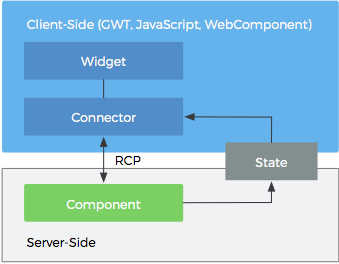
\includegraphics[width=\linewidth]{schema.png}
	\caption{Interacción Vaadin}\label{fig:schema}
\end{figure}




En este proyecto la pieza central que será la encargada de comunicarse con el conector será un componente abstracto que implementa \emph{Vaadin} para llevar a cabo esta finalidad.

Este componente consta de dos partes, por un lado tiene una clase que extiende de \emph{AbstractJavaScriptComponent} (Figura~\ref{fig:componenteVaadin}~,~Línea 2) que será la pieza que posea el contexto para comunicarse con el conector, además, en esta parte se especificarán todos los ficheros Javascript u hojas de estilo que sean necesarios (Figura~\ref{fig:componenteVaadin}~,~Línea 1). Por otro lado el estado de dicho componente, que se encargará de asegurar la integridad de los elementos que existen dentro del componente y extenderá de \emph{JavaScriptComponentState} (Figura~\ref{fig:estadoComponenteVaadin}~,~Línea 1).

\begin{figure}[!tb]
	\centering
	\begin{lstlisting}[language=Java]
	@JavaScript({ "connector.js" })
	public class Component extends AbstractJavaScriptComponent {
		public Component(String content) {
			getState().content = content;
		}
		
		@Override
		protected ComponentState getState() {
			return (ComponentState) super.getState();
		}
	}\end{lstlisting}
	\caption{Componente Vaadin}
	\label{fig:componenteVaadin}
\end{figure}


\begin{figure}[!tb]
	\centering
	\begin{lstlisting}[language=Java]
	public class ComponentState	extends JavaScriptComponentState {
		public String content;
	}\end{lstlisting}
	\caption{Estado Componente Vaadin}
	\label{fig:estadoComponenteVaadin}
\end{figure}


La comunicación del componente con el conector se puede realizar de varias formas, las más comunes son:
\begin{itemize}
	\item  Cambiando el estado del componente, ya que se ejecutará automáticamente una llamada en el conector por dicho cambio(Figura~\ref{fig:conectorDesc}~,~Líneas 6-8).
	\item  Haciendo una llamada al conector mediante una función previamente publicada (Figura~\ref{fig:callfunction}~,~Línea 1). De esta forma se puede elegir la función a la que llamar pasando una serie de parámetros.
\end{itemize}

\begin{figure}[!tb]
	\centering
	\begin{lstlisting}[language=JavaScript]
	callFunction("updateState",content);\end{lstlisting}
	\caption{Llamada al conector}
	\label{fig:callfunction}
\end{figure}



\subsubsection{Javascript Connector}	


El conector es el encargado de comunicarse con ambos lados, es decir, con el proyecto Java y el framework Javascript.

Se empieza con una cabecera, que declara la correspondencia del conector con el componente abstracto Javascript, bajo la nomenclatura \emph{window}+dirección+nombre del conector, y después se especifica el conector (Figura~\ref{fig:conectorDesc}~,~Línea 1).

El conector se compone principalmente de una función que se ejecuta cuando el estado del Componente en Vaadin cambia (Figura~\ref{fig:conectorDesc}~,~Líneas~4-6). Además, se le pueden añadir todas las funciones necesarias para el correcto funcionamiento (Figura~\ref{fig:conectorDesc}~,~Líneas~8-10). Como se puede observar en la Figura~\ref{fig:conectorDesc}~,~Línea~3, se crea un componente, este componente se correspondería, aplicando el caso al que se utilizará posteriormente en el proyecto, a \emph{GoJS}.


\begin{figure}[!tb]
	\centering
	\begin{lstlisting}[language=JavaScript]
	window.urlPaquete_connector = function() {
	
		var mycomponent = 
		new mylibrary.MyComponent(this.getElement());
		
		this.onStateChange = function() {
			mycomponent.content = this.getState().content;
		}
		
		this.updateState = function(content){
			mycomponent.content = content;
		}
	}\end{lstlisting}
	\caption{Conector}
	\label{fig:conectorDesc}
\end{figure}

En conclusión, se ha explicado un ejemplo de interacción del componente Vaadin con un Framework Javascript.